\documentclass[10pt,a4paper]{article}
\usepackage[T1]{fontenc}
\usepackage{newtxtext,newtxmath}
\usepackage[margin=19mm,headheight=20pt,headsep=8mm,footskip=12mm]{geometry}
\usepackage{amsmath,mathtools}
\usepackage{graphicx}
\usepackage{xcolor}
\usepackage{microtype}
\usepackage{titlesec}
\usepackage[most]{tcolorbox}
\usepackage{fancyhdr}
\usepackage{hyperref}
\usepackage{float}
\usepackage{needspace}

\definecolor{navy}{HTML}{163247}
\definecolor{teal}{HTML}{237C78}
\definecolor{copper}{HTML}{B94B32}
\definecolor{mist}{HTML}{F2F6F5}
\definecolor{rulegray}{HTML}{D8E1E3}
\definecolor{bodygray}{HTML}{45545C}

\hypersetup{colorlinks=true,linkcolor=teal,urlcolor=teal,pdftitle={BARNOS PART},pdfauthor={}}
\setlength{\parindent}{0pt}
\setlength{\parskip}{4.5pt plus 1pt minus 1pt}
\setlength{\emergencystretch}{2em}
\renewcommand{\arraystretch}{1.15}

\titleformat{\section}{\large\bfseries\color{navy}}{}{0pt}{}[\vspace{2pt}{\color{rulegray}\titlerule}]
\titlespacing*{\section}{0pt}{10pt}{5pt}
\titleformat{\subsection}{\normalsize\bfseries\color{teal}}{}{0pt}{}
\titlespacing*{\subsection}{0pt}{7pt}{2pt}

\pagestyle{fancy}
\fancyhf{}
\fancyhead[L]{\small\bfseries\color{navy} BARNOS PART}
\fancyhead[R]{\small\color{bodygray} Fixed-bed methanation}
\fancyfoot[L]{\small\color{bodygray} Coupled axial balances}
\fancyfoot[R]{\small\color{navy}\thepage}
\renewcommand{\headrulewidth}{0.4pt}
\renewcommand{\footrulewidth}{0pt}
\makeatletter
\renewcommand{\headrule}{\hbox to\headwidth{\color{rulegray}\leaders\hrule height \headrulewidth\hfill}}
\makeatother

\newtcolorbox{keyequation}[1][]{
  enhanced,breakable,colback=mist,colframe=mist,boxrule=0pt,
  borderline west={2pt}{0pt}{teal},left=8pt,right=8pt,top=5pt,bottom=5pt,
  before skip=5pt,after skip=7pt,#1}
\newtcolorbox{runbox}[1][]{
  enhanced,colback=navy,colframe=navy,boxrule=0pt,
  borderline west={2.5pt}{0pt}{copper},left=9pt,right=9pt,top=6pt,bottom=6pt,
  before skip=5pt,after skip=5pt,#1}

\begin{document}
\thispagestyle{fancy}

\vspace*{2mm}
{\fontsize{27}{30}\selectfont\bfseries\color{navy} BARNOS PART\par}
\vspace{4pt}
{\color{copper}\rule{32mm}{2.2pt}}\par
\vspace{5pt}
{\small\color{bodygray} Governing balances and plotted axial profiles for a reduced CO methanation model.}\par

\section{Model basis}
The bed is treated as a steady, one-dimensional plug-flow reactor. The reduced network retains CO methanation and water-gas shift (WGS):
\[
\begin{aligned}
\mathrm{CO+3H_2} &\longrightarrow \mathrm{CH_4+H_2O} && (r_2),\\
\mathrm{CO+H_2O} &\longrightarrow \mathrm{CO_2+H_2} && (r_{\mathrm W}).
\end{aligned}
\]
At each position, the reduced M4 kinetics give net rates \(r_2\) and \(r_{\mathrm W}\) from local temperature and partial pressures \(p_i=y_iP\). Rates are in \(\mathrm{mol\,kg_{cat}^{-1}\,s^{-1}}\), flows \(F_i\) in \(\mathrm{mol\,s^{-1}}\), and \(a\) is catalyst activity. Integration uses catalyst mass \(W\). For uniform loading \(\rho_B\) in a tube of cross-section \(A_c=\pi D_t^2/4\),
\[
W=\rho_B A_c z,\qquad z=\frac{W}{\rho_B A_c},\qquad W_{\mathrm{tot}}=\rho_B A_cL.
\]

A steady mole balance over a catalyst slice \(dW\) gives \(dF_i/dW=a\sum_j\nu_{ij}r_j\), where \(a\) is catalyst activity. Written for the modeled species:
\[
\begin{aligned}
\frac{dF_{\mathrm{CO}}}{dW}&=-a(r_2+r_{\mathrm W}), &
\frac{dF_{\mathrm{H_2}}}{dW}&=a(-3r_2+r_{\mathrm W}),\\
\frac{dF_{\mathrm{CH_4}}}{dW}&=ar_2, &
\frac{dF_{\mathrm{H_2O}}}{dW}&=a(r_2-r_{\mathrm W}),\\
\frac{dF_{\mathrm{CO_2}}}{dW}&=ar_{\mathrm W}, &
\frac{dF_{\mathrm{N_2}}}{dW}&=0.
\end{aligned}
\]

\section{Temperature from the energy balance}
For a differential slice, reaction heat raises the gas sensible enthalpy; heat transfer to the wall removes heat when the gas is hotter than the wall. Thus
\[
\sum_i F_iC_{p,i}\frac{dT}{dW}
=a\left[r_2(-\Delta H_2)+r_{\mathrm W}(-\Delta H_{\mathrm W})\right]
-\frac{Ua_w}{\rho_B}(T-T_w).
\]
Dividing by the gas heat-capacity flow gives the temperature equation integrated by the solver:
\begin{keyequation}
\[
\boxed{\displaystyle
\frac{dT}{dW}=
\frac{a\left[r_2(-\Delta H_2)+r_{\mathrm W}(-\Delta H_{\mathrm W})\right]
-\dfrac{Ua_w}{\rho_B}(T-T_w)}{\sum_iF_iC_{p,i}}}
\]
\end{keyequation}
Here \(a_w=4/D_t\) is the cylindrical heat-transfer area per bed volume. The formulation uses exothermic heats \(-\Delta H_2=206\) and \(-\Delta H_{\mathrm W}=41\ \mathrm{kJ\,mol^{-1}}\). The current implementation uses constant heat capacities and these constant reaction enthalpies.

\Needspace{16\baselineskip}
\section{Pressure from the Ergun equation}
The Ergun pressure gradient combines viscous resistance (first term) and inertial resistance (second term):
\[
\frac{dP}{dz}=-\left[
\frac{150\mu(1-\varepsilon_b)^2u_s}{D_p^2\varepsilon_b^3}
+\frac{1.75\rho_g(1-\varepsilon_b)u_s^2}{D_p\varepsilon_b^3}
\right].
\]
The reacting-gas properties are recalculated locally:
\[
u_s=\frac{F_{\mathrm{tot}}RT}{PA_c},\qquad
\rho_g=\frac{P\overline M}{RT},\qquad
\overline M=\sum_i y_iM_i,\qquad y_i=\frac{F_i}{F_{\mathrm{tot}}}.
\]
Since \(dz/dW=1/(\rho_BA_c)\), the pressure equation in the solver's catalyst-mass coordinate is
\begin{keyequation}
\[
\boxed{\displaystyle
\frac{dP}{dW}=-\frac{1}{\rho_BA_c}\left[
\frac{150\mu(1-\varepsilon_b)^2u_s}{D_p^2\varepsilon_b^3}
+\frac{1.75\rho_g(1-\varepsilon_b)u_s^2}{D_p\varepsilon_b^3}
\right]}
\]
\end{keyequation}
Pressure is integrated in Pa; the kinetic partial pressures are evaluated in bar. The pressure loss is coupled to reaction because the local flow, composition, temperature, and density change down the bed.

\section{Integrated solution and plotting}
The numerical problem is the coupled initial-value system
\[
\frac{d\mathbf y}{dW}=\mathbf f(\mathbf y),\qquad
\mathbf y(W)=
\begin{bmatrix}\mathbf F(W)^{\mathsf T}&T(W)&P(W)\end{bmatrix}^{\mathsf T},\qquad
\mathbf y(0)=
\begin{bmatrix}\mathbf F_0^{\mathsf T}&T_0&P_0\end{bmatrix}^{\mathsf T},
\quad 0\le W\le W_{\mathrm{tot}}.
\]
The code integrates this system with the stiff Radau method and samples the solution at 401 evenly spaced catalyst-mass locations. The plotted coordinates are \(z_j=W_j/(\rho_BA_c)\), \(T_j=T(W_j)\), and \(P_{j,\mathrm{bar}}=P(W_j)/10^5\). CO conversion is calculated as
\[
X_{\mathrm{CO}}(W)=1-\frac{F_{\mathrm{CO}}(W)}{F_{\mathrm{CO},0}}.
\]
Differentiating this definition and substituting the CO balance gives
\[
\frac{dX_{\mathrm{CO}}}{dW}
=\frac{a(r_2+r_{\mathrm W})}{F_{\mathrm{CO},0}}.
\]
Therefore, the figures show samples of the integrated profiles, not a separate closed-form solution for \(T(z)\) or \(P(z)\).

\begin{runbox}
{\small\color{white}\textbf{Plotted demonstration case.}\quad
\(D_t=0.127\,\mathrm m\), \(L=0.3048\,\mathrm m\), \(\rho_B=750\,\mathrm{kg\,m^{-3}}\), \(\varepsilon_b=0.40\), \(D_p=3\,\mathrm{mm}\), \(\mu=2.5\times10^{-5}\,\mathrm{Pa\,s}\), \(U=10\,\mathrm{W\,m^{-2}\,K^{-1}}\); \(T_0=T_w=623.15\,\mathrm K\), \(P_0=5\,\mathrm{bar}\), and feed ratio CO:H\(_2\):N\(_2\)=1:4:25 at \(0.05\,\mathrm{mol\,s^{-1}}\). Several geometry, feed, transport, and heat-transfer inputs remain assumed; this run is illustrative, not experimental validation.}
\end{runbox}

\vspace{1pt}
{\scriptsize\color{bodygray}Equation basis: Subah and Somo formulation, Sections 3, 6, and 7. Numerical implementation: \texttt{src/methanation/reactor.py}; plotting: \texttt{src/methanation/reporting.py}.}

\clearpage
\thispagestyle{fancy}
{\Large\bfseries\color{navy} CO conversion along the catalyst bed\par}
\vspace{3pt}{\color{copper}\rule{22mm}{1.6pt}}\par
\vspace{8pt}
\begin{center}
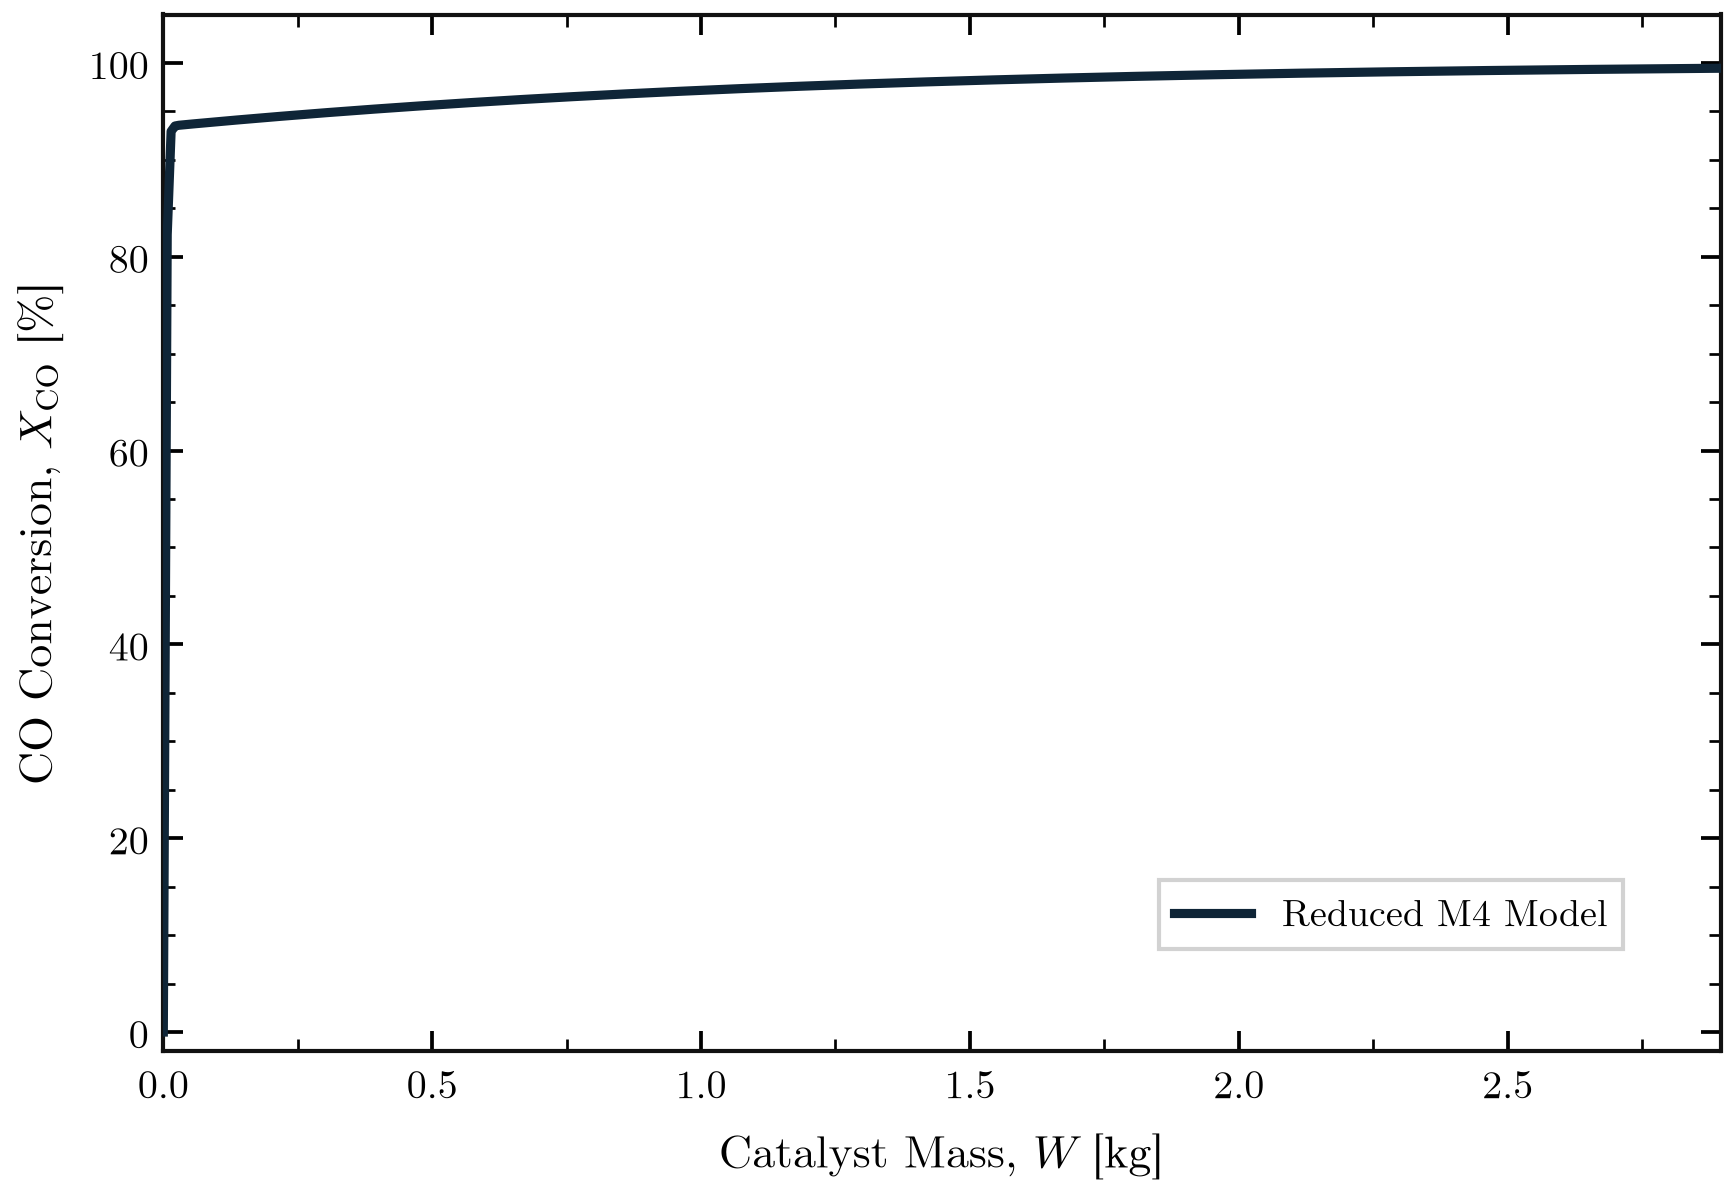
\includegraphics[width=0.96\linewidth,height=0.69\textheight,keepaspectratio]{../results/assumed_base_case/co_conversion_vs_catalyst_mass.png}
\end{center}
\begin{center}\small\textbf{Figure 1.} Reduced M4 model prediction of CO conversion versus catalyst mass for the demonstration case.\end{center}
\begin{keyequation}
\small The calculated outlet conversion is \(99.45\%\) for this assumed configuration. This curve is a model demonstration, not an experimental fit or validation result.
\end{keyequation}

\clearpage
\thispagestyle{fancy}
{\Large\bfseries\color{navy} Temperature and pressure along the bed\par}
\vspace{3pt}{\color{copper}\rule{22mm}{1.6pt}}\par
\vspace{8pt}
\begin{center}
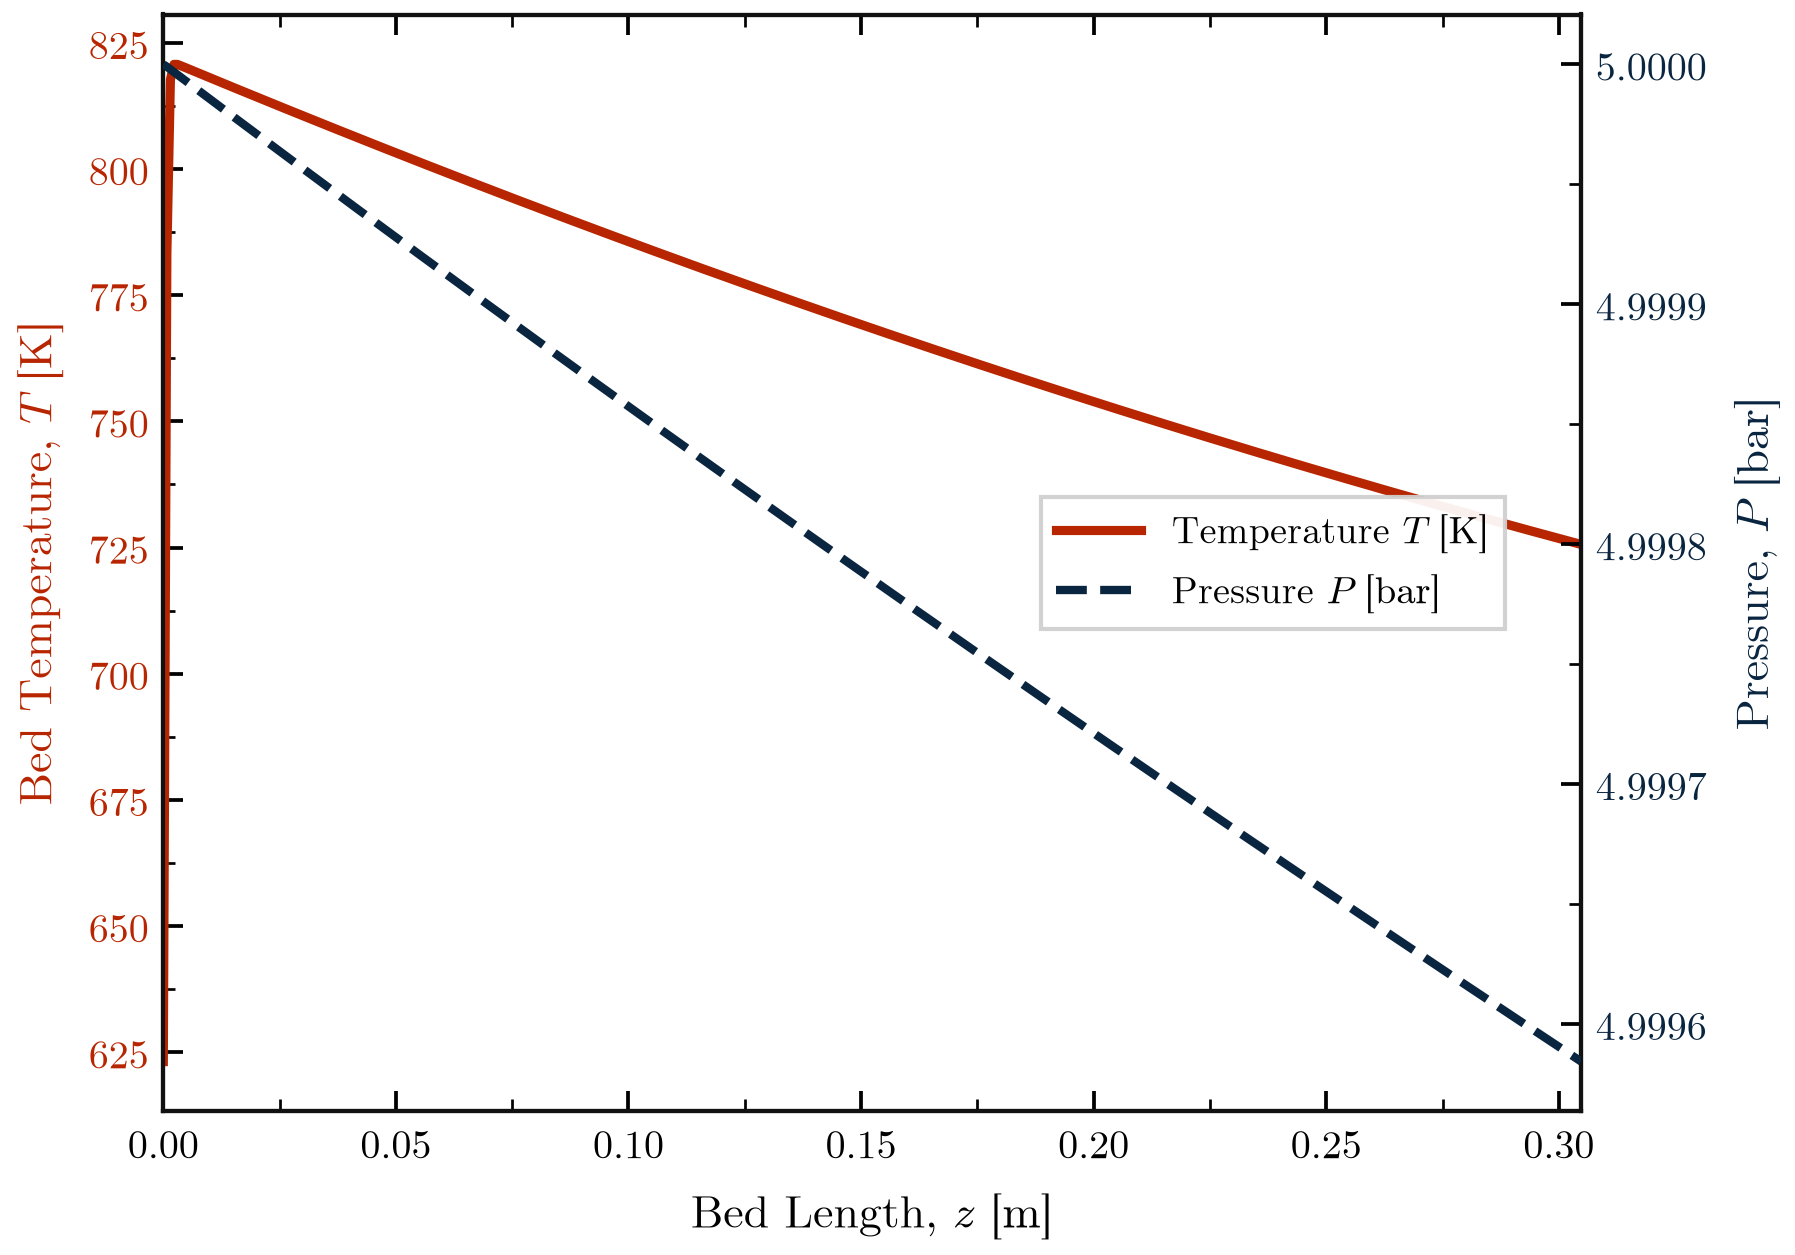
\includegraphics[width=0.96\linewidth,height=0.69\textheight,keepaspectratio]{../results/assumed_base_case/temperature_and_pressure_vs_bed_length.png}
\end{center}
\begin{center}\small\textbf{Figure 2.} Integrated temperature and Ergun pressure profiles versus bed length.\end{center}
\begin{keyequation}
\small Temperature peaks at \(820.7\,\mathrm K\) near \(z=0.0023\,\mathrm m\), then reaches \(725.6\,\mathrm K\) at the outlet. Pressure falls from \(5.0000\) to \(4.9996\,\mathrm{bar}\) (about \(41.6\,\mathrm{Pa}\)). The plotted pressure axis is tightly auto-scaled, so the visible line exaggerates this small relative drop.
\end{keyequation}

\end{document}


